\chapter{SPI sučelje mikrokontrolera STM32L4}
	Komponente senzorske pločice FERSAT-a, odnosno AD pretvornik ADS131M08 i temperaturni senzori ADT7301 komuniciraju s PDH računalom putem sučelja SPI. S obzirom da se pri razvoju programske potpore PDH računala koriste \textit{Low-Level} biblioteke, za ispravnu implementaciju upravljačkih programa nužno je razumijevanje strukture i načina rada SPI periferije izabranog mikrokontrolera. U nastavku ovog poglavlja dan je općeniti opis SPI protokola i opis SPI periferije mikrokontrolera STM32L4.
	
	\section{SPI protokol}
		\textit{Serial Peripheral Interface} (SPI) sinkrono je serijsko komunikacijsko sučelje, razvijeno u tvrtki Motorola \citep{wiki:spi}. Uobičajeno se koristi za povezivanje računala ili mikrokontrolera s brzom periferijom i senzorima na manjim udaljenostima, s obzirom da omogućava brzine do nekoliko desetaka Mbit/s. Podaci se prenose između jedne upravljačke jedinice \engl{master} i više upravljanih jedinica \engl{slave} korištenjem četiri prijenosne linije: SCLK (\textit{Serial Clock}), MISO (\textit{Master Input Slave Output}), MOSI (\textit{Master Output Slave Input}) i CS (\textit{Chip Select}, ponekad se naziva i \textit{Slave Select}). Signal takta pogoni \textit{master}, a pomoću linije CS \textit{master} odabire koji \textit{slave} smije komunicirati preko linija MISO i MOSI. Slika \ref{fig:spi} prikazuje tipičan način spajanja uređaja SPI sučeljem, u konfiguraciji jednog \textit{master} uređaja i tri \textit{slave} uređaja.
		
		\begin{figure}[htb]
			\centering
			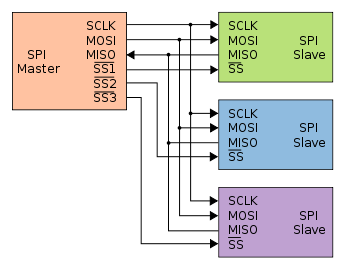
\includegraphics[height=7cm]{slike/spi.png}
			\caption{Povezivanje uređaja SPI sučeljem}
			\label{fig:spi}
		\end{figure}
	
		Postoje 4 temeljna načina rada \engl{modes} SPI sučelja, a razlikuju se po polaritetu signala takta \engl{Clock Polarity, CPOL} i bridu takta tijekom kojeg \textit{master} čita podatak \engl{Clock Phase, CPHA}.
		
	\section{Struktura SPI periferije STM32L4}
		Slika \ref{fig:stm32l4_spi} prikazuje blok dijagram SPI periferije porodice mikrokontrolera STM32L4 \citep{stm32l4}.
	
		\begin{figure}[htb]
			\centering
			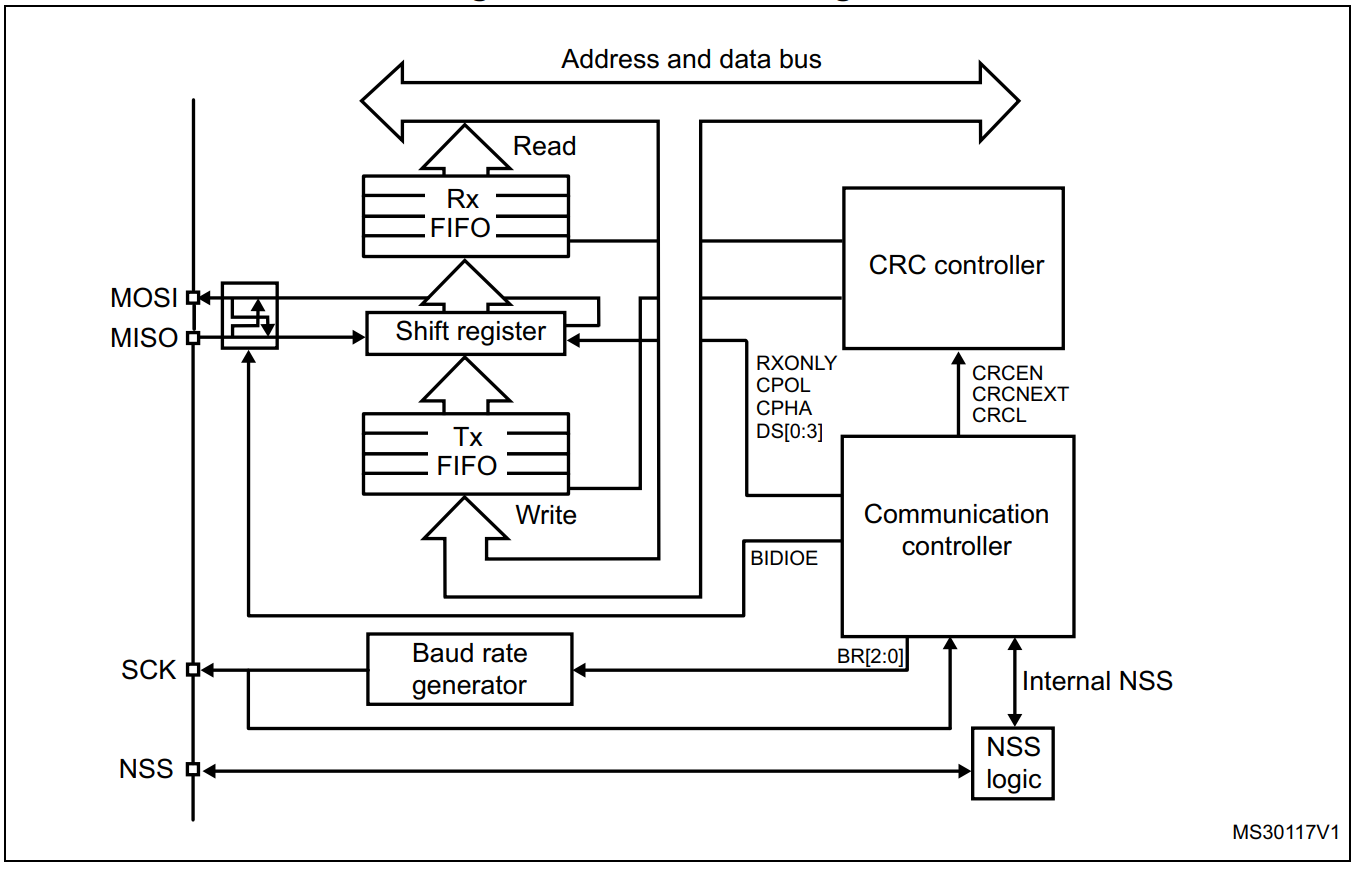
\includegraphics{slike/STM32L4_SPI_blok_dijagram.png}
			\caption{Blok dijagram SPI periferije STM32L4}
			\label{fig:stm32l4_spi}
		\end{figure}
	
		Primanje podatka odvija se na način da riječ koja se prima po MISO liniji prvo ulazi u posmačni registar \engl{shift register}, pri čemu se posmiče za jedno mjesto svaki period SPI takta. Kada je primljena cijela riječ, ona se na sljedeći brid takta prebacuje na kraj reda Rx FIFO, pri čemu se postavlja zastavica RXNE (\textit{Receiver Not Empty}) u SPI registru stanja (SPIx\_SR). Prvom podatku u redu programski se može pristupiti preko SPI podatkovnog registra (SPIx\_DR). Čitanje ovog registra automatski čisti zastavicu RXNE ukoliko je red popunjen manje od četvrtine maksimalnog kapaciteta.
		
		Slanje podatka odvija se na sličan način. Riječ upisana u SPIx\_DR sprema se na kraj reda Tx FIFO. Prva riječ u redu prebacuje se u posmačni registar, te se izlazni bit pri svakom posmaku šalje po liniji MOSI. Ako Tx FIFO sadrži manje podataka od pola svog kapaciteta, postavlja se zastavica TXE (\textit{Transmitter Empty}). Postavljanje te zastavice signalizira programu da se sljedeća riječ može upisati u red.
		
		Važno je naglasiti da SPIx\_DR nije fizički registar, već se radi o virtualnom registru koji služi za pristup redovima Rx FIFO i Tx FIFO. Pisanje u ovaj registar umeće podatak na kraj reda Tx FIFO, a čitanje sadržaja registra vraća prvi podatak u redu Rx FIFO. Oba reda su veličine 32 bita, odnosno mogu primiti 4 8-bitne riječi. Nivo popunjenosti, tj. broj 8-bitnih riječi u redu može se dobiti čitanjem bitova FTLVL[1:0] za Tx FIFO, odnosno FRLVL[1:0] za Rx FIFO u SPIx\_SR. 
		
		SPI kontroler može raditi s duljinama riječi od 4 do 16 bita. U izradi ovog rada korištena je duljina riječi 8 bita.
		
		Kontroler omogućuje hardversko izračunavanje CRC zaštitnog koda. Ova je mogućnost nakon reseta isključena, no može se omogućiti postavljanjem bita CRCEN u registru SPIx\_CR1. Tada će pogreška u prijenosu koju otkrije CRC biti signalizirana postavljanjem zastavice CRCERR u SPIx\_SR.
		
	\section{Postupak slanja i primanja podataka}
		%TODO: inicijalizacija?
		
		SPI sučelje može funkcionirati u nekoliko načina rada s obzirom na smjer komunikacije. Ti načini rada su: \textit{Full Duplex Master, Full Duplex Slave, Half Duplex Master, Half Duplex Slave, Simplex Receive Only} i \textit{Simplex Transmit Only}. U upravljačkim programima izrađenim u sklopu ovog rada korišten je način rada \textit{Full Duplex Master}, pa će zato u nastavku ovog potpoglavlja biti opisan postupak kojeg upravljački program mora izvršiti za ispravnu komunikaciju u tom načinu rada.
		
		Važno je znati da je u \textit{Full Duplex Master} načinu rada signal SPI takta određen slanjem podataka. SPI kontroler počinje generirati signal takta upisom prve riječi podatka u podatkovni registar, te generira takt dok sve riječi nisu poslane. Ako je zadnja riječ poslana i nema novih riječi u redu Tx FIFO, kontroler prestaje s generiranjem takta do sljedećeg upisa u podatkovni registar. \\
		
		Upravljački program mora slijediti sljedeću proceduru\footnote{Ova procedura je prilagođena verzija procedure opisane u priručniku mikrokontrolerske porodice STM32F4 \citep[str.~887]{stm32f4}.}:
		\begin{enumerate}
			\item Omogućiti SPI postavljanjem bita SPE u registru SPIx\_CR1.
			\item Upisati prvu riječ za slanje u podatkovni registar.
			\item Čekati dok se ne postavi zastavica TXE i zatim upisati sljedeću riječ u podatkovni registar. Čekati dok se ne postavi zastavica RXNE i zatim pročitati riječ iz podatkovnog registra. Ponavljati ovaj korak do (uključivo) predzadnje pročitane riječi.
			\item  Čekati dok se ne postavi zastavica RXNE i pročitati zadnju riječ iz podatkovnog registra.
		\end{enumerate}
	
		Čekanje zastavice TXE prilikom upisa druge riječi nije obavezno jer će ona sigurno biti postavljena, odnosno Tx FIFO sigurno može primiti dvije 8-bitne riječi. Međutim, čekanje je potrebno za svaki sljedeći upis.
	
		%TODO disable procedura?
		
		Tijekom uhodavanja SPI sučelja mikrokontrolera STM32F4 i sklopa ADT7301, uočena je greška u implementaciji HAL biblioteke za rad s SPI periferijom kada je SPI u \textit{Receive Only} načinu rada. Naime, u navedenom načinu rada potrebno je očistiti SPE bit točno jedan ciklus SPI takta nakon primitka predzadnje riječi, kako bi se spriječilo da uređaj koji šalje podatak inicira prijenos nove riječi \citep[str.~894]{stm32f4}. HAL funkcija \lstinline|HAL_SPI_TransmitReceive()| čisti SPE bit tek nakon primitka zadnje riječi, zbog čega senzor šalje još jednu riječ, pa ukupna duljina prijenosa iznosi 24 bita umjesto 16. Također, funkcija čeka da se sklopovski očisti zastavica RXNE prije nego što završi s izvođenjem, a s obzirom da se zadnja riječ nikad ne pročita, zastavica uvijek ostaje postavljena. Zbog toga funkcija uvijek čeka do isteka \textit{timeouta}, što nije poželjno ponašanje. No, to nije predstavljalo problem u daljnem tijeku izrade ovog rada, jer su za razvoj korištene LL biblioteke i \textit{Full Duplex} način rada.
		
		